\chapter{Progettazione e tecnologie}
\label{cap:progettazione-codifica}

\intro{In questo capitolo }\\

\section{Tecnologie e strumenti}
\label{sec:tecnologie-strumenti}

Di seguito viene data una panoramica delle tecnologie e strumenti presi in considerazione per lo sviluppo del prototipo. L'analisi ha valutato compatibilità, licenza, facilità d'integrazione, costi e capacità di security testing specifiche per modelli generativi. Gli strumenti e le tecnologie esaminate includono:

\begin{itemize}
    \item \textbf{PromptFoo} -- piattaforma di testing per LLM con supporto a test automatizzati e integrazione CI/CD.
    \item \textbf{PyRIT} -- tool open-source per l'identificazione e mitigazione dei rischi sui modelli generativi.
    \item \textbf{LangFuse} -- piattaforma di osservabilità e valutazione di LLM.
    \item \textbf{DeepEval / DeepTeam} -- framework di valutazione e tool di red teaming per benchmark e safety testing.
    \item \textbf{Garak} -- scanner di vulnerabilità per modelli generativi focalizzato su attacchi pratici (prompt injection, jailbreak, leakage).
    \item \textbf{Giskard} -- piattaforma di red teaming automatizzato con opzioni SaaS e libreria Python.
    \item \textbf{Galileo} -- piattaforma di osservabilità con SDK, utile per monitoraggio ma meno orientata al security testing.
    \item \textbf{LakeraGuard} -- suite di sicurezza commerciale per modelli, include test come il Gandalf test.
    \item \textbf{Tecnologie di base} -- Python, Docker, Git/GitHub, CI/CD (GitHub Actions), librerie ML (PyTorch, Hugging Face), e strumenti di logging/monitoring.
\end{itemize}

Questa panoramica ha guidato la selezione degli strumenti adottati per il prototipo, privilegiando soluzioni open-source facilmente integrabili nell'ambiente di sviluppo e con funzionalità mirate al security testing dei modelli generativi.

\subsection{Strumenti analizzati}
Durante le prime due settimane di Stage è stato condotto uno studio preliminare su diversi strumenti di security testing per AI generativa. Di seguito viene fornita la matrice di valutazione dei tools e una breve descrizione di ciascuno strumento analizzato.

\begin{figure}[!h]
    \centering
    % includegraphics is redefined in config/thesis-config.tex to prepend
    % the images/ folder, so here we only pass the filename
    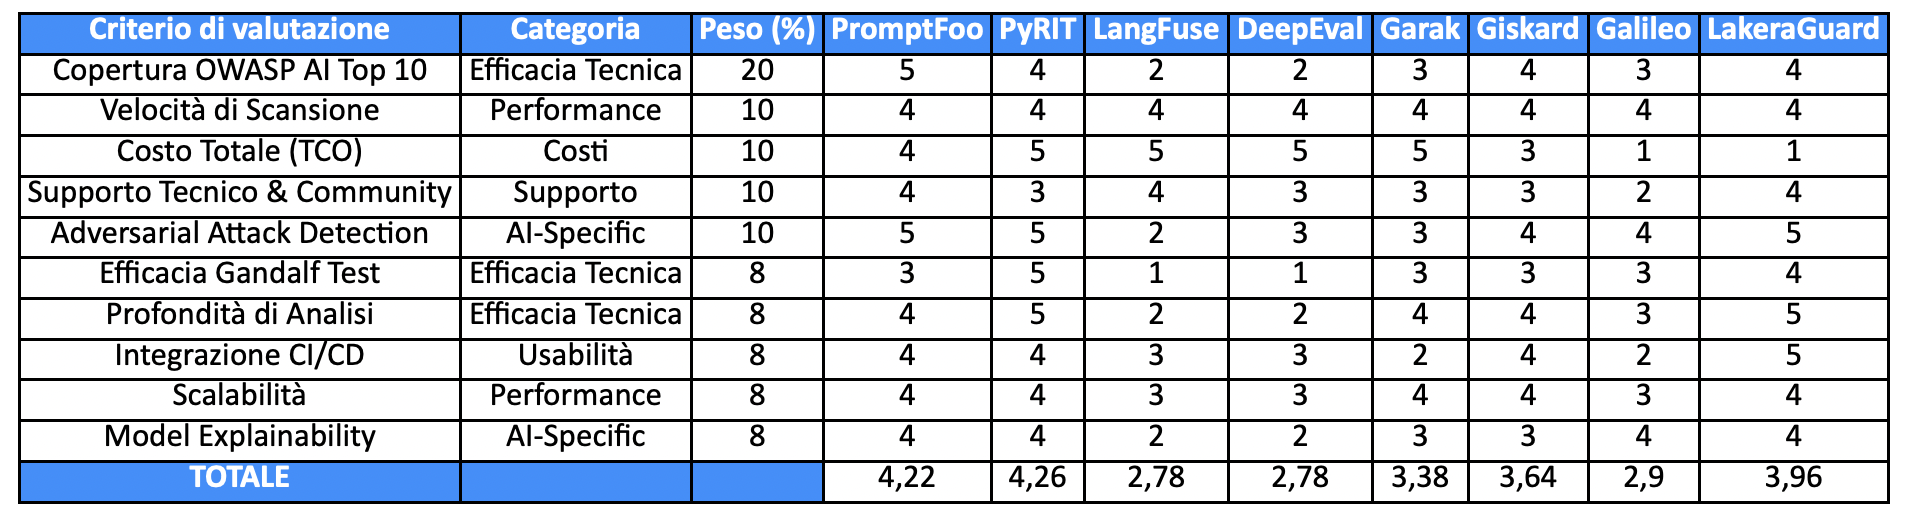
\includegraphics[width=1.0\columnwidth]{matrix.png}
    \caption{Matrice di Valutazione degli Strumenti Analizzati}
\end{figure}

\subsubsection*{PromptFoo}
PromptFoo è una piattaforma di testing per modelli di linguaggio che consente agli sviluppatori di creare, eseguire e gestire test automatizzati per valutare le prestazioni, l'affidabilità e la sicurezza dei loro modelli di linguaggio naturale. Offre funzionalità come la creazione di casi di test personalizzati, l'integrazione con pipeline CI/CD e report dettagliati sui risultati dei test.
Questo tool è stato tenuto in molta considerazione in quanto offre funzionalità specifiche per il testing delle vulnerabilità OWASP top 10 per AI generativa, obbiettivo principale del progetto di stage.

\subsubsection*{PyRIT}
PyRIT è uno tool open-source progettato da Azure Microsoft per l'identificazione e la mitigazione dei rischi associati all'uso di modelli di intelligenza artificiale generativa. PyRIT è stato creato per valutare modelli di AI per potenziali vulnerabilità di sicurezza, bias e problemi di conformità, fornendo raccomandazioni su come migliorare la sicurezza e l'affidabilità dei modelli.\\


\subsubsection*{LangFuse}
LangFuse è una piattaforma open-source per la valutazione e l'osservazione delle applicazioni che utilizzano intelligenza artificiale generativa. La piattaforma è integrata con diversi modelli di linguaggio naturale e permette l'utilizzo tramite cloud o in self host. Langfuse offre inoltre un LLM playground per testatre i modelli che aveva catturato la mia attenzione all'inizio del progetto. Tuttavia il tool non offre una vera e propria funzionalità di security testing, focus del progetto di stage.

\subsubsection*{DeepEval / DeepTeam}
DeepEval è un framework open-source per la valutazione e il benchmarking dei modelli di intelligenza artificiale generativa. DeepEval non fornisce funzionalità specifiche per il testing dei modelli. Per ovviare a questa mancanza è stato creato un tool di testing basato su DeepEval chiamato DeepTeam, un tool di red teaming. Tuttavia, DeepTeam non ha un focus sulle vulnerabilità OWASP in quanto si concentra sul testing delle safety guidelines.

\subsubsection*{Garak}
Garak è uno scanner di vulnerabilità per modelli di intelligenza artificiale generativa open-source creato da NVIDIA per facilitare il testing dei modelli. Il focus di Garak sta nei metodi di attacco specifici per far fallire in modo imprevisto una LLM o un sistema di dialogo. Garak testa diverse vulnerabilità tra cui allucinazioni, data leakage, prompt injection, jailbreaks ecc.

\subsubsection*{Giskard}
Giskard è una piattaforma di red teaming automatizzato per testare, valutare ed analizzare modelli di intelligenza artificiale generativa. Esistono due metodi di utilizzo di Giskard: Come servizio HUB a pagamento o come libreria Python open-source da installare localmente. La libreria fornita è però fortemente limitata nelle funzionalità rispetto al servizio HUB in quanto incentrata sulla ricerca.

\subsubsection*{Galileo}
Galileo è una piattaforma che permette la valutazione e osservazione di applicazioni basate su AI generativa. Galileo offre SDK in Python e TypeScript per integrarlo direttamente nei propri progetti. Galileo è molto flessibile per quanto riguarda il deploy e viene utilizzato da molte aziende di rilievo. Nonostante ciò la piattaforma non offre funzionalità specifiche per il security testing, focus di questo progetto, ed è a pagamento.

\subsubsection*{LakeraGuard}
LakeraGuard è una piattaforma di sicurezza per modelli di intelligenza artificiale che aiuta gli sviluppatori a proteggere i loro modelli da minacce e vulnerabilità. Offre funzionalità come la scansione delle vulnerabilità, la gestione delle patch e il monitoraggio delle minacce in tempo reale.\\
Essendo l'azienda svizzera Lakera la creatrice del gandalf test, focus principale delle prime settimane del progetto di stage, il tool da loro creato è stato uno dei primi ad essere analizzato. 
Tuttavia il tool out of the box fa già quello che lo stage chiede di implementare quindi non ha suscitato uno studio approfondito in quanto avrebbe reso superfluo lo sviluppo del prototipo.\\
Inoltre è un tool a pagamento che offre un tier gratuito il quale è però limitato a 10000~richieste \gls{api} al mese, limite che avrebbe reso difficile l'utilizzo futuro del tool.


\subsection{Strumenti utilizzati}
Di seguito viene data una panoramica delle tecnologie e strumenti utilizzati per lo sviluppo del prototipo.

\subsubsection*{Python + PyRIT}
Python è un linguaggio di programmazione versatile e ampiamente utilizzato, particolarmente adatto per lo sviluppo di applicazioni backend. PyRIT è uno strumento open-source progettato da Azure Microsoft per l'identificazione e la mitigazione dei rischi associati all'uso di modelli di intelligenza artificiale generativa. Insieme, Python e PyRIT forniscono un ambiente potente per lo sviluppo e la sicurezza delle applicazioni AI.DA AGGIUNGERE PERCHÉ USATO

\subsubsection*{React}
React è una libreria JavaScript per la creazione di interfacce utente, sviluppata da Facebook. È ampiamente utilizzata per costruire applicazioni web dinamiche e reattive. La sua architettura basata su componenti consente agli sviluppatori di creare interfacce utente modulari e riutilizzabili, semplificando il processo di sviluppo.DA AGGIUNGERE PERCHÉ USATO

\subsubsection*{MongoDB}
MongoDB è un database NoSQL orientato ai documenti, progettato per gestire grandi volumi di dati non strutturati. Utilizza un modello di dati flessibile basato su BSON, che consente agli sviluppatori di archiviare e recuperare informazioni in modo efficiente. MongoDB è particolarmente adatto per applicazioni che richiedono scalabilità e prestazioni elevate.DA AGGIUNGERE PERCHÉ USATO

\section{Progettazione}
\label{sec:progettazione}

\subsection{Progettazione Backend} %**************************
Descrizione struttura backend \& spiegazione infrastruttura di persistenza dei dati

\subsection{Progettazione Frontend} %**************************
Descrizione pagine frontend


\section{Design Pattern utilizzati}

STRATEGY PER CAMBIARE AL VOLO IL TIPO DI TEST ( DATASET E SCORER PROMPT )

